

% Introduce Topology

\begin{frame}{$n$-cell Concept}
 \begin{block}{Concept of \emph{$n$-cell}}
  \begin{itemize}
   \item Sub-$k$-cells of an $n$-cell
  \end{itemize}
  \vspace*{-0.3cm}
  \begin{center}
    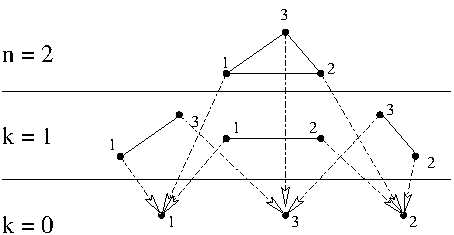
\includegraphics[width=0.37\textwidth]{triangle-layers} \hspace{0.2cm}
    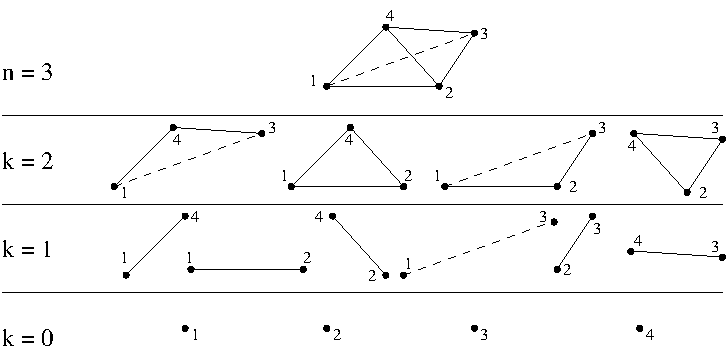
\includegraphics[width=0.59\textwidth]{tetrahedron-layers}
  \end{center}
 \end{block}

 \visible<1->{
 \begin{block}{Separation of Geometry and Topology}
  \begin{itemize}
    \item Geometry: Euclidian space, coordinate system
    \item Topology: Connection between points (lines, triangles, etc.)
  \end{itemize}
 \end{block}
 \vspace*{0.3cm}
 }
\end{frame}




\begin{frame}[fragile]
\frametitle{ViennaGrid Datastructure}
 \begin{block}{Datastructure Requirements}
   \begin{itemize}
    \item Don't store boundary $k$-cells unnecessarily
    \item Fast local iteration on $k$-cells
   \end{itemize}
 \end{block}

  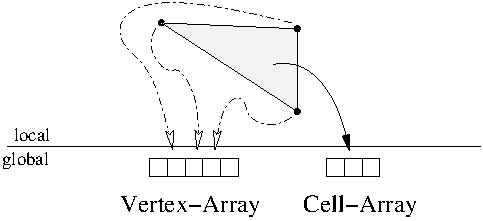
\includegraphics[width=0.45\textwidth]{storage-vglob-cglob} \hspace*{0.3cm}
  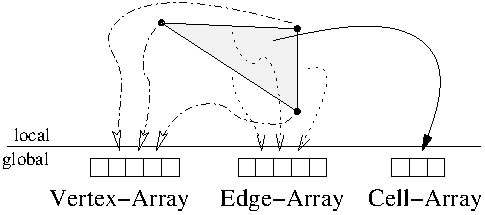
\includegraphics[width=0.49\textwidth]{storage-vglob-eglob-cglob} \\

 \visible<1->{
 \vspace*{0.3cm} 
 \begin{tabular}{|l|r|r|r|}
  \hline
         & \scriptsize Amount      & \scriptsize Mem/Obj.         & \scriptsize Total Mem. \\
  \hline
  \tiny Vertices & \footnotesize 4913 & \footnotesize 24 B & \footnotesize 115 KB \\
  \hline
  \tiny Edges   & \footnotesize 31024 & \footnotesize 16 B & \footnotesize 485 KB \\
  \hline
  \tiny Facets  & \footnotesize 50688 & \footnotesize 48 B & \footnotesize 2376 KB \\
  \hline
  \tiny Cells   & \footnotesize 24576 & \footnotesize 112 B & \footnotesize 2688 KB \\
  \hline
  \scriptsize \textbf{Total}  &       &     & \footnotesize  \textbf{5664 KB} \\
  \hline
 \end{tabular}
 \begin{tabular}{|l|r|r|r|}
  \hline
         & \scriptsize Amount      & \scriptsize Mem/Obj.         & \scriptsize Total Mem. \\
  \hline
  \tiny Vertices & \footnotesize 4913 & \footnotesize 24 B & \footnotesize 115 KB \\
  \hline
  \tiny Edges   & \footnotesize 0 & - & \footnotesize 0 KB \\
  \hline
  \tiny Facets  & \footnotesize 0 & - & \footnotesize 0 KB \\
  \hline
  \tiny Cells   & \footnotesize 24576 & \footnotesize 32 B & \footnotesize 768 KB \\
  \hline
  \scriptsize \textbf{Total}  &       &     & \footnotesize  \textbf{883 KB} \\
  \hline
 \end{tabular}
 \vspace*{0.5cm}
 }
\end{frame}




\begin{frame}[fragile]{$n$-cell Implementation}

 \begin{block}{Implementation of \lstinline|element_t|}
  \begin{itemize}
   \item Recursive inheritance from boundary layer of dimension $n-1$
   \item Tag dispatching to enable/disable topological layers
  \end{itemize}
  \vspace*{-0.2cm}
  \begin{center}
    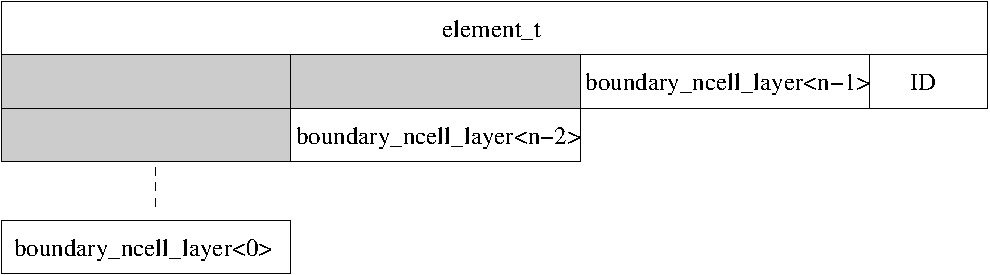
\includegraphics[width=0.77\textwidth]{recursive-inheritance}
  \end{center}
 \end{block}

 %\visible<2->{
 \begin{lstlisting}[basicstyle=\scriptsize\ttfamily]
  template <typename ConfigType, typename ElementTag>
  class element_t :
    public boundary_ncell_layer<ConfigType, ElementTag, ElementTag::dim-1>,
    public result_of::element_id_handler<ConfigType, ElementTag>::type
 \end{lstlisting}
 \vspace*{0.3cm}
 %}
\end{frame}

